\documentclass[10pt,a4paper]{article}
\usepackage[utf8]{inputenc}
\usepackage[T1]{fontenc}
\usepackage[margin=0.75in]{geometry}
\usepackage{parskip}
\usepackage{booktabs}
\usepackage{float}
\usepackage{amsmath}
\usepackage{caption}
\usepackage{tikz}
\usetikzlibrary{arrows.meta,positioning,shapes.geometric}
\usepackage{pgfplots}
\pgfplotsset{compat=1.16}
\usepgfplotslibrary{groupplots}

% Signal names with subscripts
\newcommand{\vrefh}{\ensuremath{V_{\mathrm{REFH}}}}
\newcommand{\vrefl}{\ensuremath{V_{\mathrm{REFL}}}}
\newcommand{\vtap}{\ensuremath{V_{\mathrm{TAP}}}}
\newcommand{\vout}{\ensuremath{V_{\mathrm{OUT}}}}
\newcommand{\vdd}{\ensuremath{V_{\mathrm{DD}}}}
\newcommand{\vssa}{\ensuremath{V_{\mathrm{SS}}}}
\newcommand{\ibias}{\ensuremath{I_{\mathrm{BIAS}}}}
\newcommand{\idd}{\ensuremath{I_{\mathrm{DD}}}}
\newcommand{\iref}{\ensuremath{I_{\mathrm{REF}}}}
\newcommand{\en}{\ensuremath{\mathrm{EN}}}
\newcommand{\dbus}{\ensuremath{D_5\text{--}D_0}}

\title{\textbf{1.8\,V Rail-to-Rail 6-Bit Buffered DAC in Sky130} \\ \large ICARUS TEAM 4: Flatline}
\author{}
\date{}
\makeatletter\renewcommand{\@maketitle}{\begin{center}{\LARGE \@title \par}\end{center}\vspace{0.5em}}\makeatother

\begin{document}

\maketitle

% ============================================================
\section{Overview}
A voltage-output, 6-bit resistor-string DAC with an integrated unity-gain output buffer, for Chipalooza Challenge \#4 in Sky130. The whole block runs from a single $1.8\,\mathrm{V}$ supply shared by the logic and analog circuitry, and the string spans the full rail ($\vrefl = \vssa$, $\vrefh = \vdd$), so the output is rail to rail: $0$ to $\tfrac{63}{64}\vdd$ ($1.772\,\mathrm{V}$ at $1.8\,\mathrm{V}$). It holds a static voltage and drives a $100\,\mathrm{k\Omega} \parallel 20\,\mathrm{pF}$ load. Existing Sky130 Chipalooza DACs are AC-only (audio), current-output (IDAC), unbuffered for $\geq 100\,\mathrm{M\Omega}$ loads (8-bit RDAC) or short-term (12-bit CDAC); this block fills the gap for a static, buffered voltage DAC.

% ============================================================
\section{Applications}
\begin{itemize}
    \item Programmable comparator thresholds and trim or calibration voltages
    \item Low-frequency set points routed across the SoC or to a pin
\end{itemize}

% ============================================================
\section{Topology}
\begin{itemize}
    \item \textbf{Resistor string:} 64 matched $\approx 1\,\mathrm{k\Omega}$ poly units from \vssa{} to \vdd{}; inherently monotonic, and ratiometric to the supply
    \item \textbf{Tap selector:} 6-level binary tree of $1.8\,\mathrm{V}$ CMOS transmission gates, one level per bit, so no decoder is needed; $\vtap = D\,\vdd/64$, $D = 0\ldots63$
    \item \textbf{Switch drivers:} logic and switches share the $1.8\,\mathrm{V}$ supply, so no level shifters are needed; two inverters per bit (and for \en{}) give the complementary gate drives
    \item \textbf{Output buffer:} two-stage op-amp at unity gain with NMOS and PMOS input pairs, so it senses taps from $0\,\mathrm{V}$ to \vdd{} (rail-to-rail input); NMOS common-source output against a $100\,\mu\mathrm{A}$ PMOS source, Miller-compensated ($45\,\mathrm{pF}$ MIM, $1.5\,\mathrm{k\Omega}$ poly); $1\,\mu\mathrm{A}$ bias mirrored to $10\,\mu\mathrm{A}$ per input pair
    \item \textbf{Enable:} \en{} low connects the buffer input to \vrefl{} (ground). Codes may change while \en{} is high; brief multi-bit glitches are expected
\end{itemize}

\begin{figure}[H]
\centering
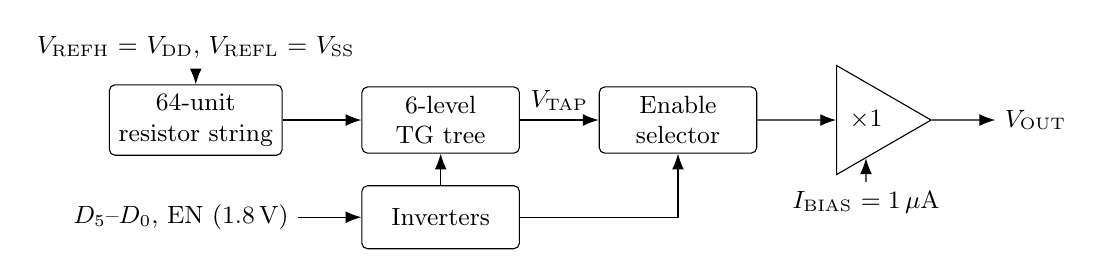
\begin{tikzpicture}[
    blk/.style={draw, rounded corners=2pt, minimum height=8mm, minimum width=20mm, align=center, font=\small},
    arr/.style={-{Latex[length=2mm]}},
    lbl/.style={font=\small}]
  \node[blk] (str) {64-unit\\resistor string};
  \node[blk, right=10mm of str] (tree) {6-level\\TG tree};
  \node[blk, right=10mm of tree] (mux) {Enable\\selector};
  \node[draw, isosceles triangle, isosceles triangle apex angle=60, minimum height=12mm, right=10mm of mux, font=\small] (buf) {$\times 1$};
  \node[blk, below=4mm of tree] (ls) {Inverters};
  \node[lbl, right=8mm of buf] (out) {\vout};
  \node[lbl, above=2mm of str] (refs) {\vrefh{} $=$ \vdd, \vrefl{} $=$ \vssa};
  \node[lbl, left=8mm of ls] (dig) {\dbus, \en{} ($1.8\,\mathrm{V}$)};
  \node[lbl, below=3mm of buf] (bias) {\ibias{} $= 1\,\mu\mathrm{A}$};
  \draw[arr] (refs) -- (str);
  \draw[arr] (str) -- (tree);
  \draw[arr] (tree) -- node[above, lbl] {\vtap} (mux);
  \draw[arr] (mux) -- (buf);
  \draw[arr] (buf) -- (out);
  \draw[arr] (dig) -- (ls);
  \draw[arr] (ls) -- (tree);
  \draw[arr] (ls.east) -| (mux.south);
  \draw[arr] (bias) -- (buf);
\end{tikzpicture}
\end{figure}

% ============================================================
\section{Pin List}
\begin{table}[H]
  \centering
  \begin{tabular}{@{}l l l@{}}
    \toprule
    \textbf{Pin} & \textbf{Function} & \textbf{Type} \\
    \midrule
    \dbus       & Data code, $D_5$ = MSB (6 harness control inputs)              & Digital in, $1.8\,\mathrm{V}$ \\
    \en         & Enable; low resets output to \vrefl{} (1 control input)        & Digital in, $1.8\,\mathrm{V}$ \\
    \vrefh      & Upper end of the string; tied to \vdd{} (no harness line)       & Internal \\
    \vrefl      & Lower end of the string; tied to \vssa{} (no harness line)       & Internal \\
    \vtap       & Unbuffered tap; test port and fallback output (shared analog line) & Analog out \\
    \vout       & Buffered DAC output (dedicated pad, requested)                 & Analog out \\
    \ibias      & $1\,\mu\mathrm{A}$ mirrored harness current                     & Bias in \\
    \vdd        & $1.8\,\mathrm{V}$ supply for logic, string and buffer (per-slot switch) & Power \\
    \vssa        & Ground                                                         & Power \\
    \bottomrule
  \end{tabular}
\end{table}

Harness resources: 7 of 24 control inputs, 0 status outputs, 1 of 4 shared analog lines, 1 dedicated pad and 1 bias current.

% ============================================================
\section{Target Specifications}
Conditions: $\vrefl = \vssa$, $\vrefh = \vdd$, load $100\,\mathrm{k\Omega} \parallel 20\,\mathrm{pF}$ (including pad, package and fixture). $1\,\mathrm{LSB} = \vdd/64 = 28.125\,\mathrm{mV}$ at $1.8\,\mathrm{V}$; errors are referred to the measured supply. Typical values are pre-layout simulation results at TT, $25\,^\circ$C, $1.8\,\mathrm{V}$.
\begin{table}[H]
  \centering
  \begin{tabular}{@{}l c c c l@{}}
    \toprule
    \textbf{Parameter} & \textbf{Min} & \textbf{Typ} & \textbf{Max} & \textbf{Unit} \\
    \midrule
    Supply \vdd{} (logic and analog)      & 1.71  & 1.8   & 1.89  & V \\
    Temperature                           & $-20$ & 25    & 110   & $^\circ$C \\
    Bias current \ibias                   & 0.8   & 1.0   & 1.2   & $\mu$A \\
    Resolution                            & --    & 6     & --    & bit \\
    Output, code 0                        & 0     & 0.0032 & --   & V \\
    Output, code 63                       & --    & 1.7707 & $\tfrac{63}{64}\vdd$ & V \\
    Absolute error, every code            & $-0.5$ & 0.11 & $+0.5$ & LSB \\
    DNL                                   & $-0.5$ & 0.13 & $+0.5$ & LSB \\
    INL (endpoint fit)                    & $-0.5$ & 0.13 & $+0.5$ & LSB \\
    Monotonicity                          & \multicolumn{3}{c}{Guaranteed} & -- \\
    Settling after a code change, $\pm 0.5\,\mathrm{LSB}$ & -- & 9.2 & 20 & $\mu$s \\
    String current \iref                  & --    & 28.0  & 40    & $\mu$A \\
    Static supply current \idd{} (incl.\ \iref) & -- & 0.17 & 0.5 & mA \\
    \bottomrule
  \end{tabular}
\end{table}

\textbf{Absolute limits:} \vdd{} $0$--$1.95\,\mathrm{V}$; every signal pin between \vssa{} and \vdd{}; \ibias{} $\leq 2\,\mu\mathrm{A}$; \vout{} must not be driven or shorted. \vout{} and \vtap{} reach the $3.3\,\mathrm{V}$ pad frame, so they need overvoltage protection (Challenge \#4 Rule 10). Sky130 device and pad ratings take precedence.

\textbf{Basis for the values:} the single $1.8\,\mathrm{V}$ supply matches the harness logic and removes the level shifters; tying the string to the rails gives a rail-to-rail range and frees the two reference lines, at the cost of a supply-ratiometric output; the NMOS output stage bottoms out about $3\,\mathrm{mV}$ above ground, which sets the code-0 error ($0.11\,\mathrm{LSB}$); $45\,\mathrm{pF}$ compensation was chosen from a $20$--$60\,\mathrm{pF}$ sweep (phase margin $71.5^\circ$ at TT and $69.0^\circ$ at SS, $110\,^\circ$C, $1.71\,\mathrm{V}$; faster than $60\,\mathrm{pF}$); the $1\,\mathrm{k\Omega}$ unit sets $28\,\mu\mathrm{A}$ of string current; $\pm 0.5\,\mathrm{LSB}$ is a common DAC target and $20\,\mu\mathrm{s}$ suits occasional threshold updates; $20\,\mathrm{pF}$ is our pad, package and fixture estimate; supply tolerance is assumed until harness documentation is published. The SF ($-20\,^\circ$C) and SS ($110\,^\circ$C) runs at $1.71\,\mathrm{V}$ stay within $\pm 0.16\,\mathrm{LSB}$ and settle in $\leq 14.1\,\mu\mathrm{s}$. All will be revisited after layout.

% ============================================================
\section{Verification Plan}
\pgfplotstableread{
code vout errlsb inllsb dnllsb
0 0.003189 113.404 0.000 -131.079
1 0.027628 -17.675 -128.606 -7.673
2 0.055537 -25.348 -133.806 -1.976
3 0.083607 -27.323 -133.309 -0.656
4 0.111713 -27.980 -131.492 -0.322
5 0.139829 -28.302 -129.341 -0.225
6 0.167948 -28.527 -127.094 -0.201
7 0.196067 -28.728 -124.822 -0.249
8 0.224185 -28.977 -122.598 -0.598
9 0.252293 -29.575 -120.723 -1.569
10 0.280374 -31.144 -119.819 1.777
11 0.308549 -29.367 -115.569 1.567
12 0.336718 -27.800 -111.529 1.202
13 0.364877 -26.598 -107.854 2.133
14 0.393062 -24.465 -103.249 3.474
15 0.421285 -20.992 -97.302 5.106
16 0.449553 -15.886 -89.723 6.579
17 0.477863 -9.307 -80.672 7.099
18 0.506188 -2.208 -71.100 6.122
19 0.534485 3.914 -62.505 3.996
20 0.562722 7.910 -56.036 1.717
21 0.590896 9.627 -51.846 0.066
22 0.619023 9.694 -49.307 -0.692
23 0.647128 9.001 -47.526 -0.690
24 0.675234 8.311 -45.743 -0.302
25 0.703350 8.010 -43.572 0.145
26 0.731479 8.155 -40.954 0.578
27 0.759621 8.733 -37.903 1.030
28 0.787775 9.763 -34.400 1.523
29 0.815942 11.286 -30.404 2.014
30 0.844124 13.300 -25.917 2.421
31 0.872317 15.721 -21.024 2.638
32 0.900516 18.359 -15.912 2.614
33 0.928715 20.973 -10.826 2.352
34 0.956906 23.325 -6.001 1.931
35 0.985085 25.255 -1.598 1.437
36 1.013251 26.692 2.312 0.950
37 1.041402 27.643 5.736 0.518
38 1.069542 28.161 8.727 0.126
39 1.097671 28.287 11.326 -0.277
40 1.125788 28.010 13.521 -0.380
41 1.153902 27.630 15.615 -0.286
42 1.182019 27.345 17.802 -0.287
43 1.210136 27.058 19.988 -0.318
44 1.238252 26.740 22.143 -0.342
45 1.266367 26.397 24.273 -0.360
46 1.294482 26.037 26.386 -0.371
47 1.322597 25.666 28.488 -0.381
48 1.350711 25.285 30.580 -0.388
49 1.378825 24.898 32.665 -0.395
50 1.406939 24.503 34.744 -0.402
51 1.435053 24.101 36.815 -0.411
52 1.463166 23.691 38.877 -0.422
53 1.491279 23.268 40.927 -0.442
54 1.519392 22.826 42.958 -0.471
55 1.547504 22.355 44.960 -0.527
56 1.575614 21.829 46.906 -0.639
57 1.603721 21.189 48.740 -0.898
58 1.631821 20.292 50.315 -1.548
59 1.659902 18.743 51.240 -3.220
60 1.687937 15.523 50.493 -7.024
61 1.715864 8.500 45.942 -14.889
62 1.743570 -6.389 33.526 -35.998
63 1.770683 -42.388 0.000 nan
}\dactt
\begin{itemize}
    \item \textbf{Remaining:} port to Xschem/ngspice and CACE for open-source sign-off; FF and FS corners and combined mismatch/PVT; layout with dummies and common-centroid inputs; DRC, LVS and PEX re-simulation over PVT; overvoltage protection on \vout{} and \vtap{}; harness switch, pad and \vtap{} line models
    \item \textbf{Silicon:} 64-code sweep over SPI with a precision DMM on \vout{} and \vdd{} (error, DNL, INL, monotonicity); \vtap{} vs.\ \vout{} to separate string and buffer errors; scope settling and glitches ($0 \leftrightarrow 63$, $31 \leftrightarrow 32$); $100\,\mathrm{k\Omega}$ and $1\,\mathrm{M\Omega}$ loads; supply, \ibias{} and temperature extremes
\end{itemize}

\begin{figure}[H]
\centering
\begin{tikzpicture}
\begin{axis}[width=\textwidth, height=7.2cm, xmin=-1, xmax=64, xtick={0,8,...,56,63},
    xlabel={Code $D$}, ylabel={$V_{\mathrm{OUT}}$ (V)}, ymin=0, ymax=1.9, ytick={0,0.3,...,1.8},
    grid=both, grid style={gray!20}, tick label style={font=\small}, label style={font=\small},
    legend cell align=left, legend style={font=\small, at={(0.02,0.97)}, anchor=north west, fill=white}]
  \addplot[red, dashed, thick, domain=0:63] {x*0.028125};
  \addlegendentry{Ideal line}
  \addplot[blue, densely dotted, thick, domain=0:63] {0.003189 + x*(1.770683-0.003189)/63};
  \addlegendentry{Endpoint line}
  \addplot[only marks, mark=*, mark size=1.3pt] table[x=code, y=vout] {\dactt};
  \addlegendentry{Simulated $V_{\mathrm{OUT}}$}
  \node[font=\small, anchor=south east] at (axis cs:63,0.05) {$1\,\mathrm{LSB} = 28.125\,\mathrm{mV}$};
\end{axis}
\end{tikzpicture}

\vspace{2mm}
\begin{tikzpicture}
\begin{axis}[width=\textwidth, height=7.2cm, xmin=-1, xmax=64, xtick={0,8,...,56,63},
    xlabel={Code $D$}, ylabel={Error ($10^{-3}$ LSB)}, ymin=-200, ymax=200, ytick={-200,-150,...,200},
    grid=both, grid style={gray!20}, tick label style={font=\small}, label style={font=\small},
    legend cell align=left, legend style={font=\small, at={(0.98,0.03)}, anchor=south east, fill=white}]
  \addplot[gray, thick, forget plot] coordinates {(-1,0) (64,0)};
  \addplot[red, thick, mark=*, mark size=1.2pt] table[x=code, y=errlsb] {\dactt};
  \addlegendentry{Accuracy: vs.\ ideal line}
  \addplot[blue, thick, mark=square*, mark size=1.1pt] table[x=code, y=inllsb] {\dactt};
  \addlegendentry{Linearity (INL): vs.\ endpoint line}
  \addplot[green!50!black, thick, mark=triangle*, mark size=1.5pt, unbounded coords=jump] table[x=code, y=dnllsb] {\dactt};
  \addlegendentry{DNL: step from $D$ to $D+1$, minus 1 LSB}
  % Error-table values and axis coordinates are in 10^{-3} LSB.
  \node[font=\footnotesize, text=red, align=left, anchor=west] at (axis cs:1.2,113)
    {Accuracy $+0.113\,\mathrm{LSB}$ at $D=0$ ($3.19\,\mathrm{mV}$ floor)};
  \node[font=\footnotesize, text=green!50!black, align=left, anchor=west] at (axis cs:2,-62)
    {DNL $-0.131\,\mathrm{LSB}$ at $0\to1$};
  \node[font=\footnotesize, text=blue, align=left, anchor=west] at (axis cs:3,-160)
    {INL $-0.134\,\mathrm{LSB}$ at $D=2$};
\end{axis}
\end{tikzpicture}

\vspace{1mm}
{\small Top: settled output versus code. Bottom: accuracy is the deviation from the ideal line; INL is the deviation from the endpoint line; DNL is the step-size error relative to $1\,\mathrm{LSB}$. One vertical-axis unit is $0.001\,\mathrm{LSB}$ ($28.1\,\mu\mathrm{V}$). The largest errors come from code 0, where the output stays $3.19\,\mathrm{mV}$ above ground. All steps are positive (minimum $24.44\,\mathrm{mV}$, at $0 \to 1$).}
\captionsetup{skip=3pt}\caption*{\footnotesize Sky130 pre-layout simulation (pinned BSIM, poly-resistor and MIM models), TT corner, $25\,^\circ$C, $1.8\,\mathrm{V}$, $100\,\mathrm{k\Omega} \parallel 20\,\mathrm{pF}$ load. The LTspice schematics were re-simulated in ngspice to export every code; code 0 and code 63 agree with the LTspice run within $0.07\,\mathrm{mV}$. Resistors are identical in this run; mismatch is assessed separately.}
\end{figure}

% ============================================================
\section{Deliverables}
\begin{itemize}
    \item Schematics, layout (GDS) and LEF views, testbenches, CACE results and DRC/LVS reports in a public Apache 2.0 repository
    \item Datasheet, bench measurement scripts and published silicon results
\end{itemize}

% ============================================================

\end{document}
